\documentclass[../main.tex]{subfiles}

\begin{document}

\section{Potential energy analysis}

\begin{figure}[ht!]
    \centering
    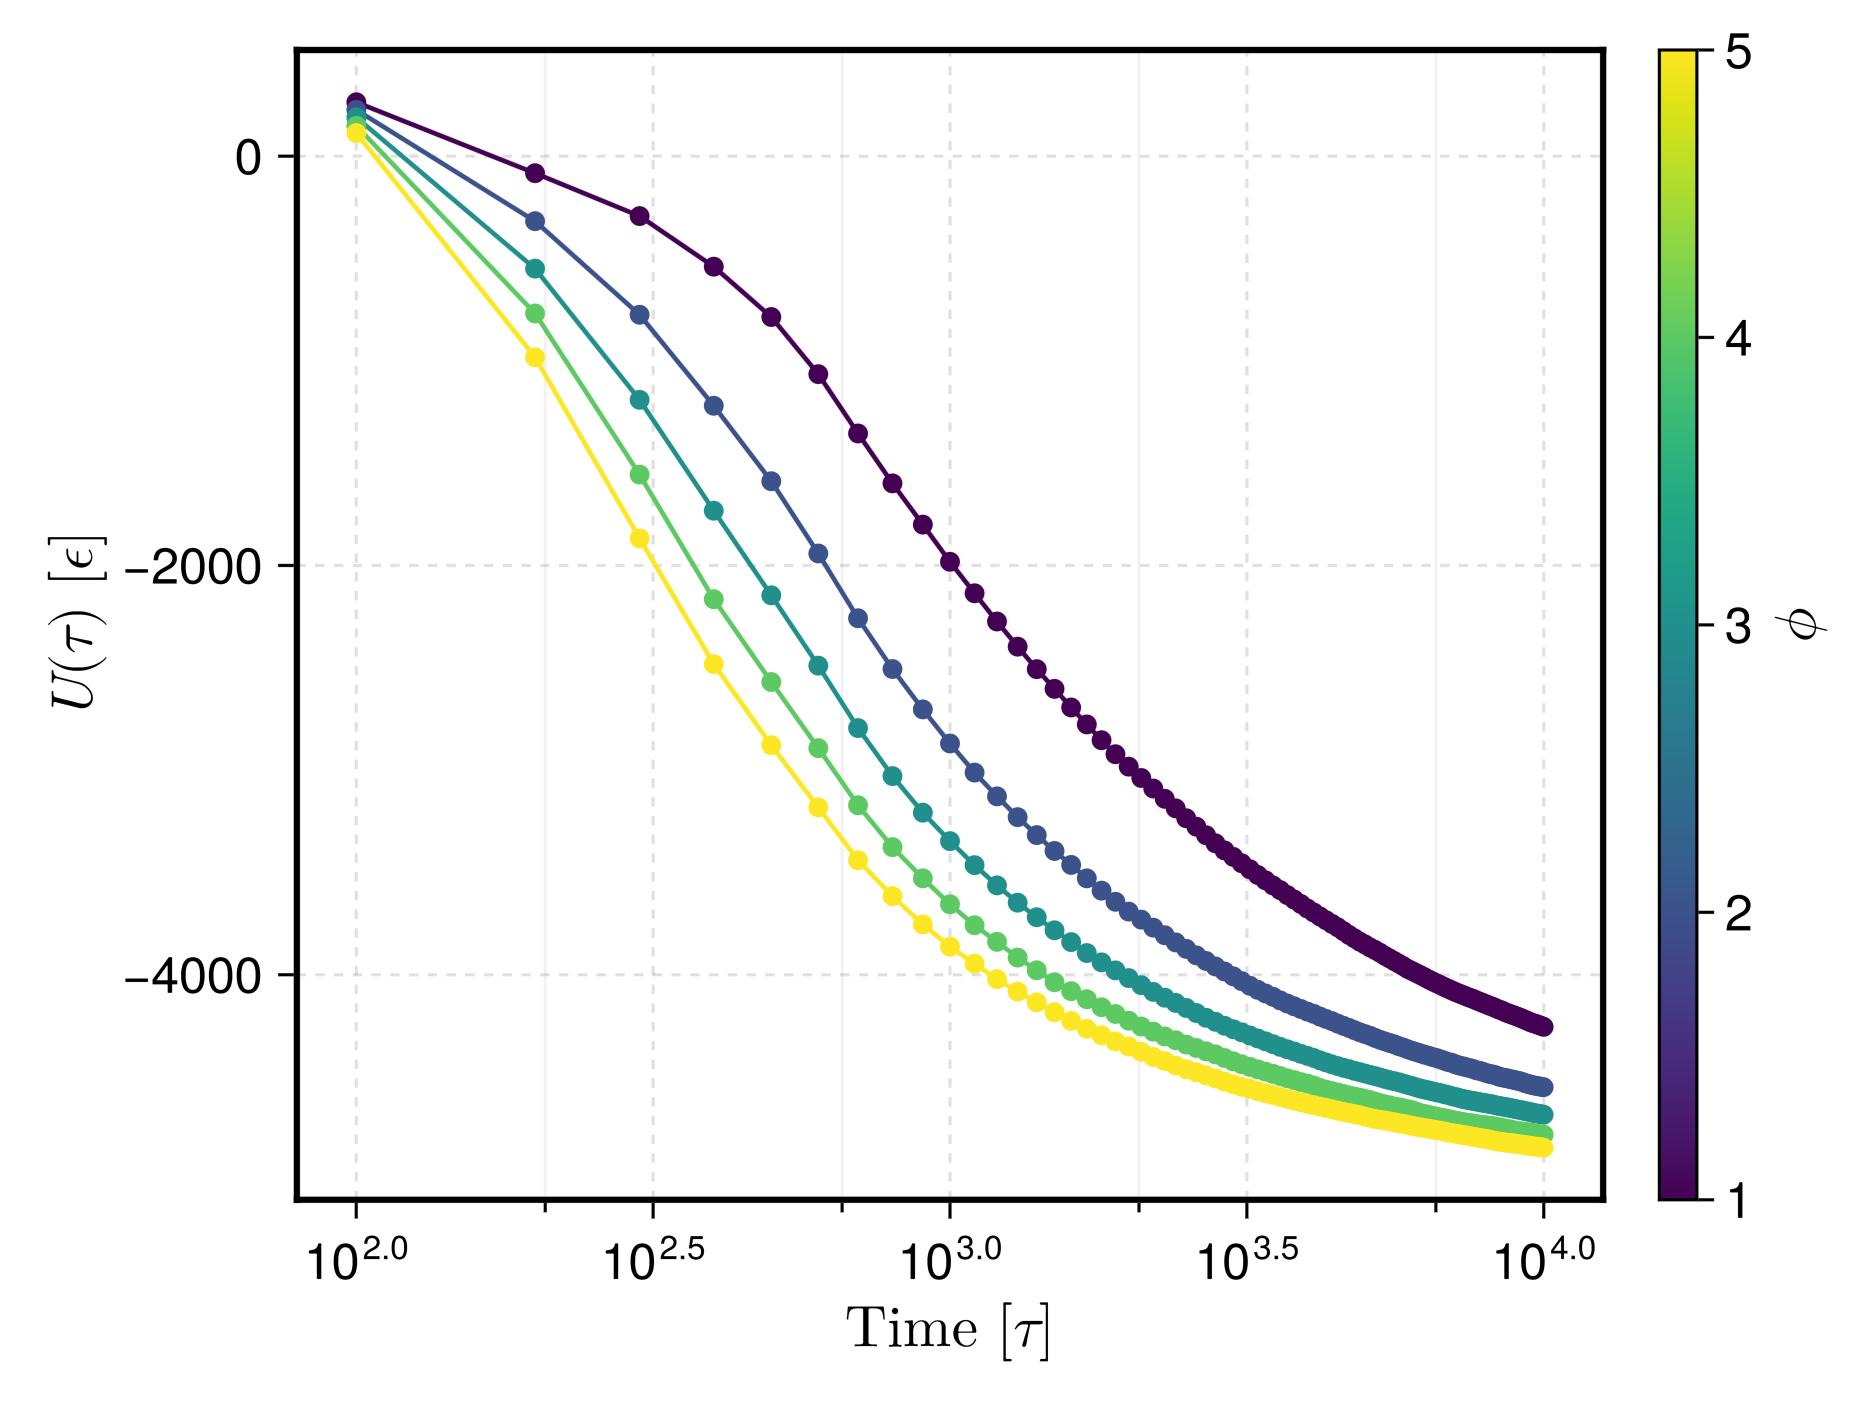
\includegraphics{../Figures/fig_PotEnergy_phiseries.png}
    \caption{
        Comparisson of the time evolution of the potential energy for systems with different packing fractions.
    }
\end{figure}

\section{Structure factor analysis}

Three length scales can be defined for the structural factor to analyze the system's structure.
The large length scale regime is characterized by the condition $10^{-1.5}\leq|\vec{q}|\leq 10^{-0.5}$.
An intermediate length scale regime is characterized by the criterion $10^{-1/2}\leq|\vec{q}|\leq 10^{1/2}$.
A small length scale regime is described as $10^{-0.5}\leq|\vec{q}|\leq 10^{1.0}$.
The three regimes are distinguished by gray, blue, and red, respectively.

\begin{figure}[ht!]
    \centering
    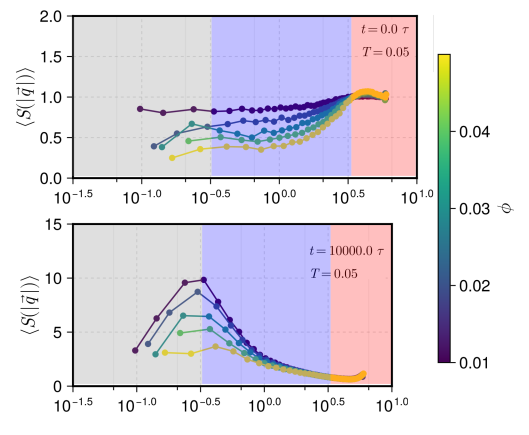
\includegraphics{../Figures/StructureFactorCompare.png}
    \caption{
        Comparisson of the structure factor for systems with different packing fractions.
        Grey area represent the large length scale, the blue area represent the intermediate length scale and the red area represent the small length scale.
        Top pannel is the initial configuration.
        The bottom panel is the final configuration after \num{10e3} time units.
    }\label{fig:structure_factor}
\end{figure}

Beginning with the structure factor of the initial condition, top panel of figure~\ref{fig:structure_factor}, at the large length scale regime, it is observed that at low packing fractions, the intensity approaches one, whereas an increase in packing fraction leads to a reduction in intensity.
The results indicates that the patchy particles at a low packing fraction are randomly and uniformly dispersed throughout the simulated box, as expected.
Nonetheless, as the packing percentage increases, large scale density variations gradually start to be suppressed.
In the intermediate length regime, the intensity of the structure factor for the system with $\phi>1$ increases towards one, while the intensity of the structure factor for the system with the lowest packing fraction remains about at 1.  
This indicates that at these length scales, the initial state for systems with $\phi>1$ begins to approximate that of an ideal gas, similar to the system with $\phi=1$.  
Furthermore, at the small length scale regime, the intensity of all structure factors approaches 1.  
This signifies that the cores of the central particles are randomly distributed within the volume of the simulation box, which displays identical initial conditions to the minimum packing percentage.

At \num{10e3} time units, the lower panel of figure~\ref{fig:structure_factor} has a little peak in the small length scale region, indicating a characteristic length.
This peak represents the average size of the patchy particle, taking into account the distance from the core's center to the surface of a patch.
At the intermediate length scale, the structure factor seemingly demonstrates a linear relationship with a negative slope as the packing percentage increases.
This outcome signifies that an increase in packing fraction causes the system to resemble a gel network.
Ultimately, at extensive length scales, the structure factor for systems with $\phi=1\%, 2\%$, and $3\%$ rapidly approaches 1, forming a peak near the transition between the large and intermediate regimes.
The pattern signifies the formation of several smaller clusters measuring around $19.86$ length units.  
Conversely, the structure factor for the systems with $\phi=4\%$ and $5\%$ does not diminish; rather, it remains roughly stable.
This feature signifies the creation of a significant, dense cluster with tightly packed substructures.

\section{Pore analysis}

The methodology implemented for these graphs involves selecting random places within the simulation box and progressively increasing the radius of a sphere until it intersects with a patchy particle.

\begin{figure}[ht!]
    \centering
    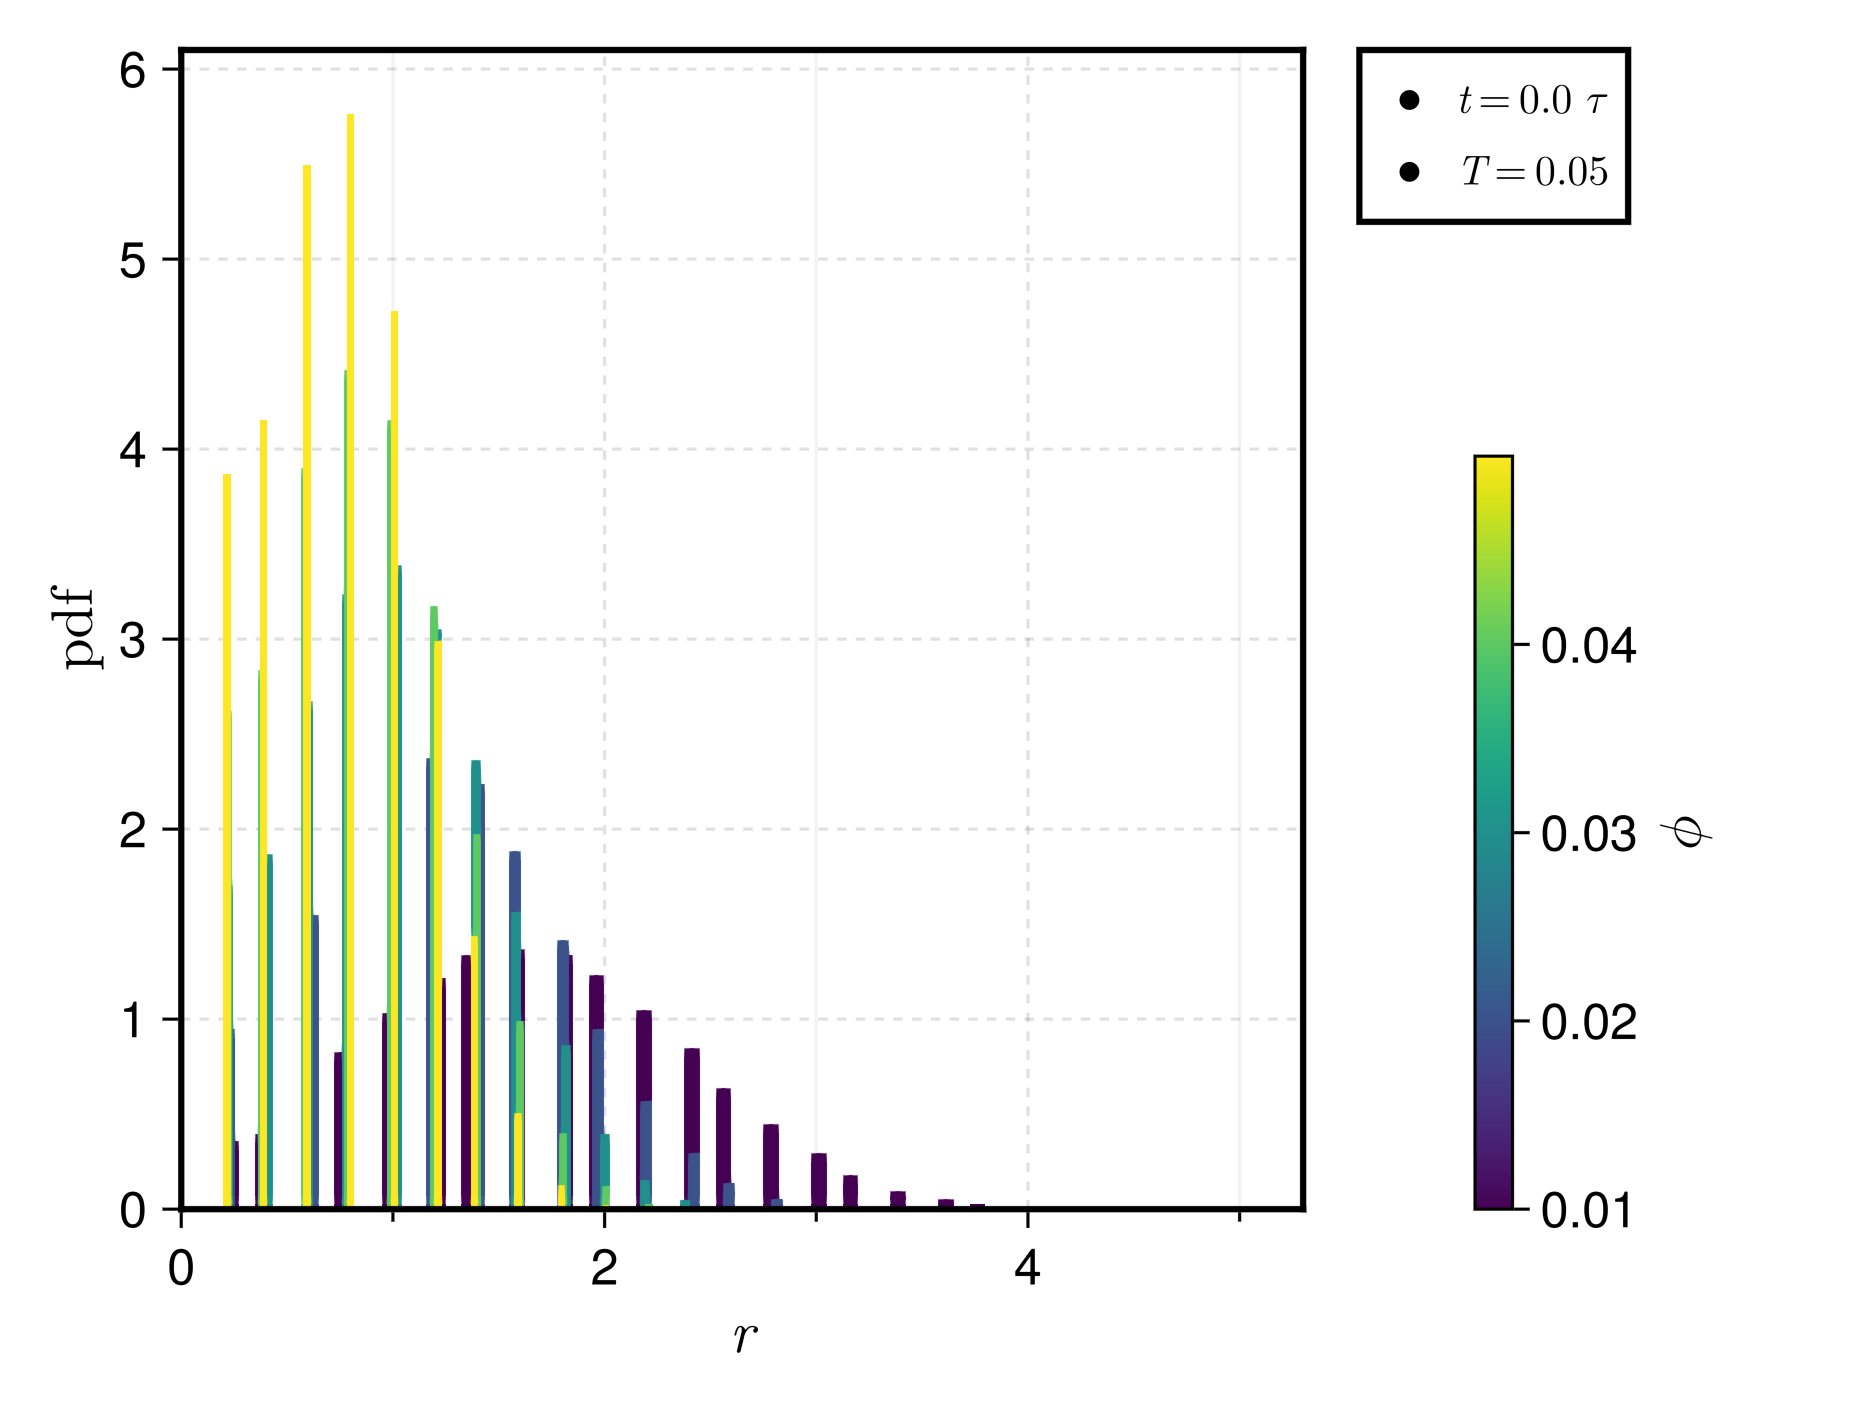
\includegraphics{../Figures/fig_pore_histogram_phiseries0.010.050.051.0500000.09.5e6_time_0.0.png}
    \caption{
        Comparisson of the distributions of the pore size for systems with different packing fractions at the initial configuration.
    }
\end{figure}

\begin{figure}[ht!]
    \centering
    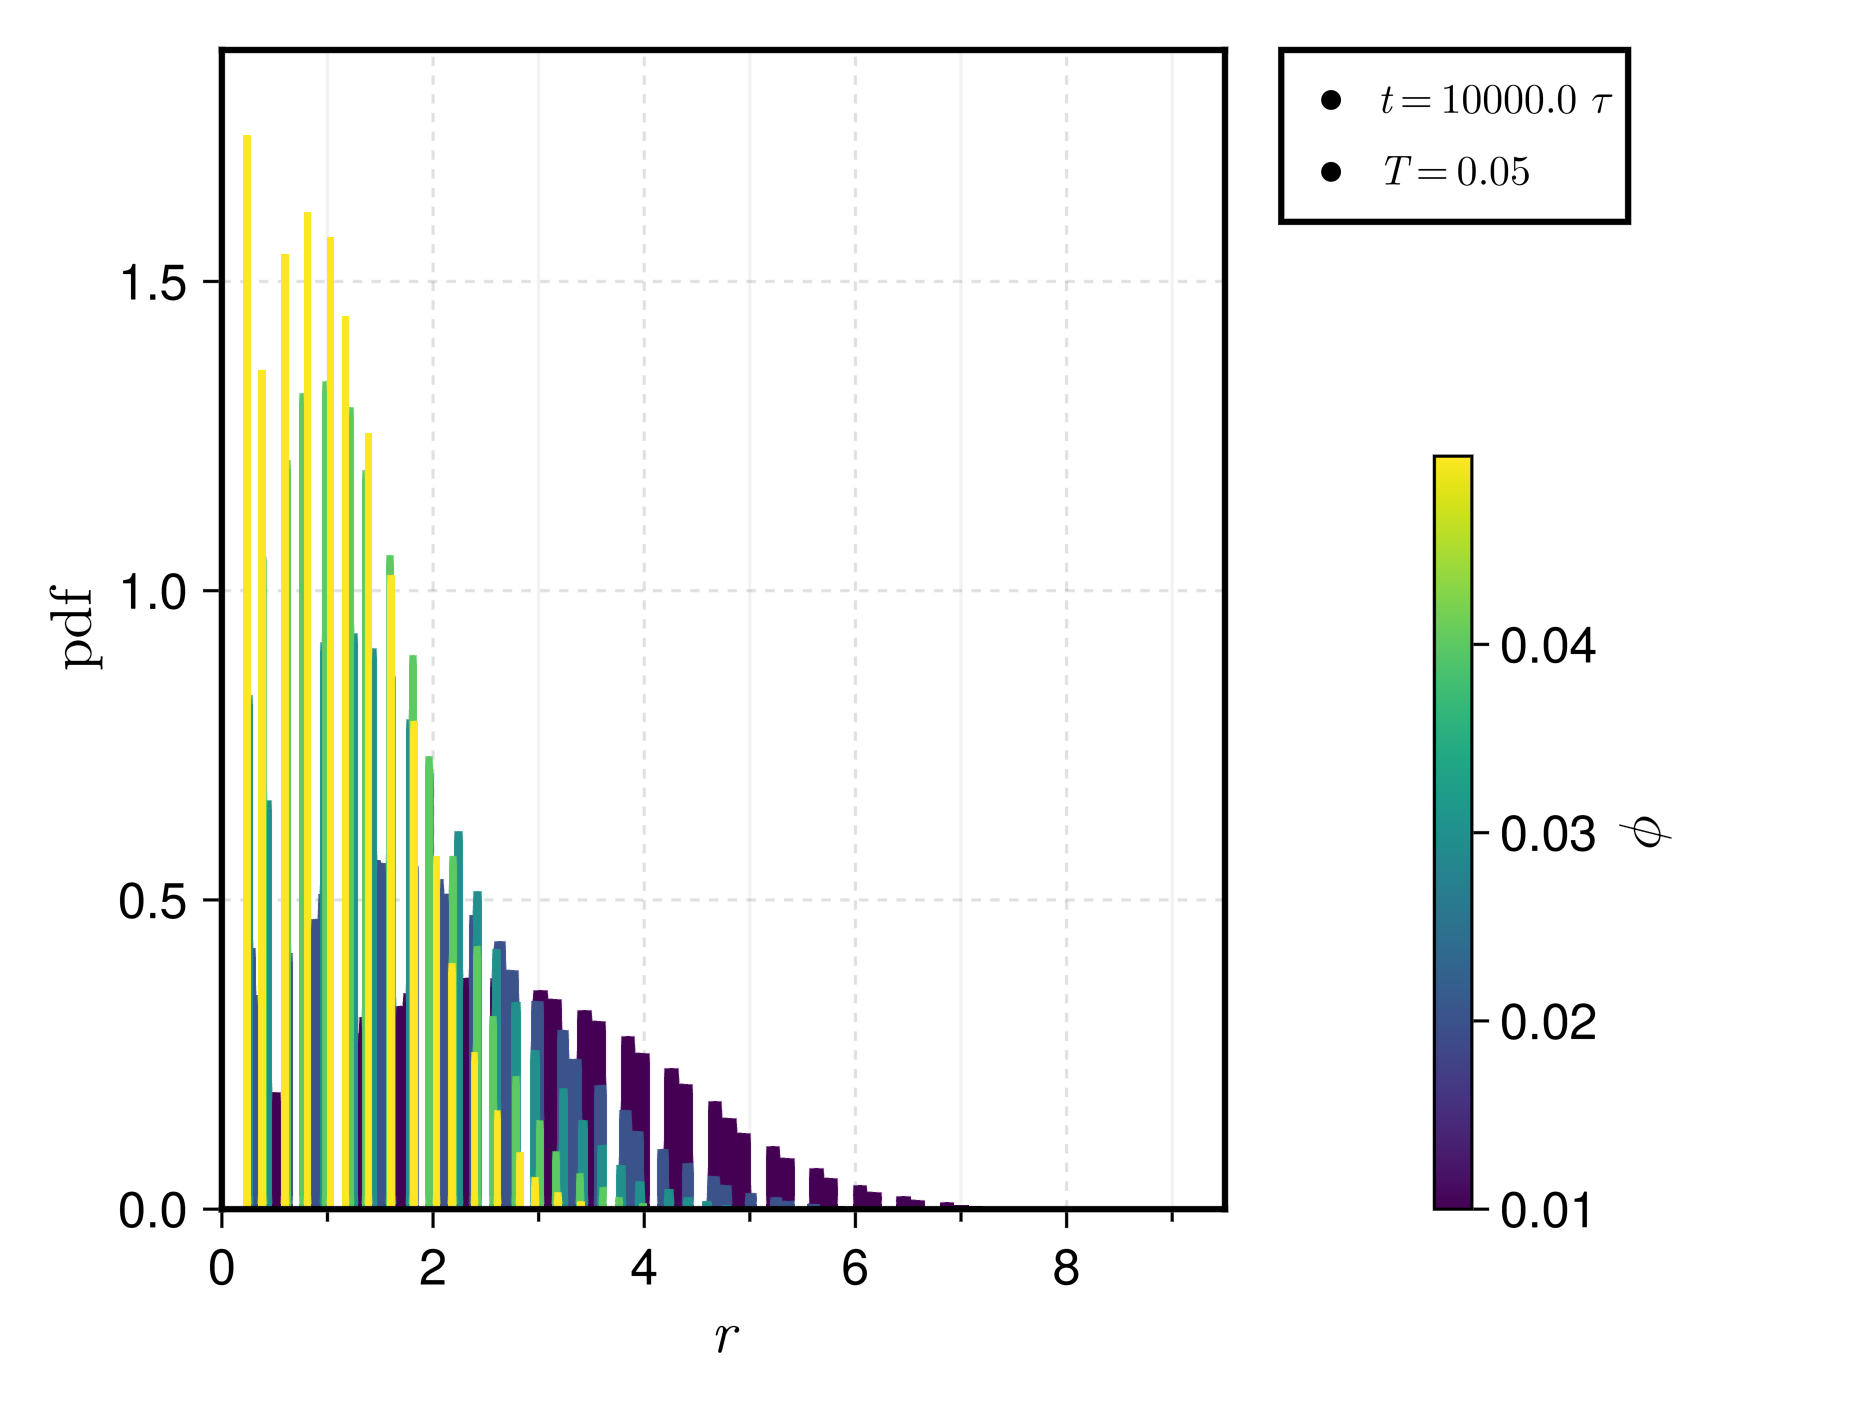
\includegraphics{../Figures/fig_pore_histogram_phiseries0.010.050.051.0500000.09.5e6_time_1.0e7.png}
    \caption{
        Comparisson of the distributions of the pore size for systems with different packing fractions after \num{10e3} time units.
    }
\end{figure}



\end{document}
